\section{Results}
\label{sec:results}

All values in this section are derived from \emph{training artifacts only} (see Section~\ref{sec:experiments}). We report primary outcomes for \Exp{01}--\Exp{03}, then place them in context using benchmark and cross-pair diagnostics generated under the same simulator semantics.

% ------------------------------------------------------------------
\subsection{Global Performance Dashboard}
% ------------------------------------------------------------------

Before unpacking each experiment family, \Cref{fig:metrics_multi_panel} provides a compact multi-metric snapshot of profitability, risk, and behavior indicators used throughout this section.

\begin{figure*}[!tbp]
\centering
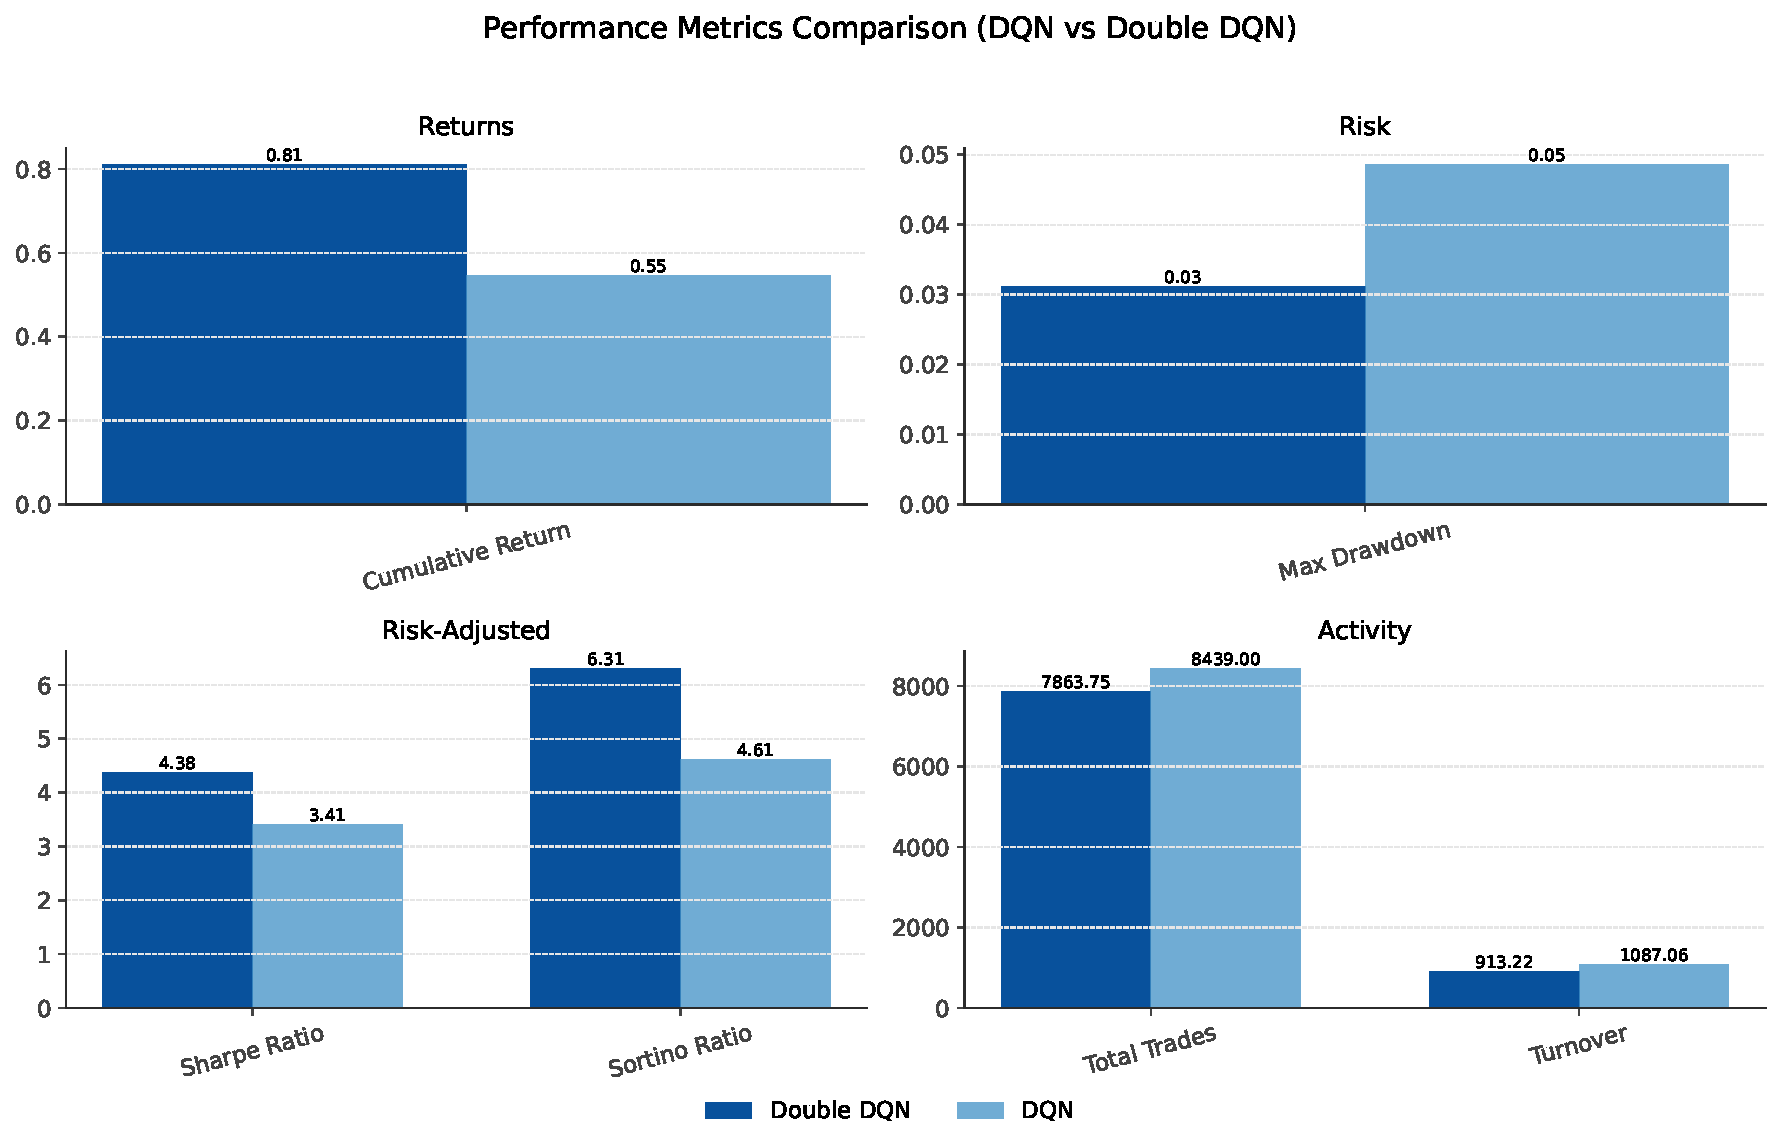
\includegraphics[width=\linewidth]{figures/metrics_multi_panel.pdf}
\caption{Multi-panel dashboard of endpoint metrics across retained experiment families, summarizing return, drawdown, risk-adjusted performance, and activity.}
\label{fig:metrics_multi_panel}
\end{figure*}

The dashboard confirms that no single configuration dominates all dimensions simultaneously: variants with stronger endpoint return often incur higher activity or weaker conservative risk summaries, reinforcing the need for objective-specific model selection.

% ------------------------------------------------------------------
\subsection{Reward Component Ablation (\Exp{01})}
% ------------------------------------------------------------------

\noindent\textbf{Objective.}
\Exp{01} progressively enables reward components to identify constructive versus destructive interactions.

We first report endpoint statistics in \Cref{tab:ablation_train}, then use distributional and trajectory views to diagnose interaction nonlinearity.

\begin{table*}[!tbp]
\centering
\caption{Reward ablation on EURUSD train split (Double DQN; see Section~\ref{sec:experiments}).}
\label{tab:ablation_train}

\begin{adjustbox}{width=\linewidth}
\begin{tabular}{lrrrrrrrr}
\toprule
\textbf{Variant} & \textbf{Sharpe} & \textbf{Sortino} & \textbf{Cum.Ret(\%)} & \textbf{MaxDD(\%)} & \textbf{WinRate(\%)} & \textbf{Turnover} & \textbf{AvgPyr} & \textbf{AvgMart} \\
\midrule
\variant{r1} & 0.412 & 0.573 & 27.79 & 10.48 & 35.18 & 1592.83 & 0.113 & 0.121 \\
\variant{r2} & 0.237 & 0.353 & 12.20 & 8.60 & 31.85 & 1741.58 & 0.187 & 0.127 \\
\variant{r3} & 0.638 & 0.979 & 41.20 & 5.44 & 31.53 & 1488.67 & 0.165 & 0.138 \\
\variant{r4} & 0.687 & 1.029 & 43.21 & 5.68 & 30.99 & 1344.47 & 0.197 & 0.144 \\
\variant{r5} & 0.589 & 0.822 & 41.74 & 4.12 & 31.07 & 1350.00 & 0.172 & 0.156 \\
\variant{r6} & 0.410 & 0.539 & 24.58 & 7.70 & 27.38 & 1200.32 & 0.132 & 0.089 \\
\variant{r7} & 0.765 & 1.117 & 57.09 & 2.31 & 33.15 & 1156.51 & 0.173 & 0.169 \\
\bottomrule
\end{tabular}
\end{adjustbox}
\end{table*}




Endpoint values already indicate interaction effects: Sharpe and cumulative return do not improve monotonically with added penalties, and several intermediate variants underperform simpler compositions.

\begin{figure}[!tbp]
\centering
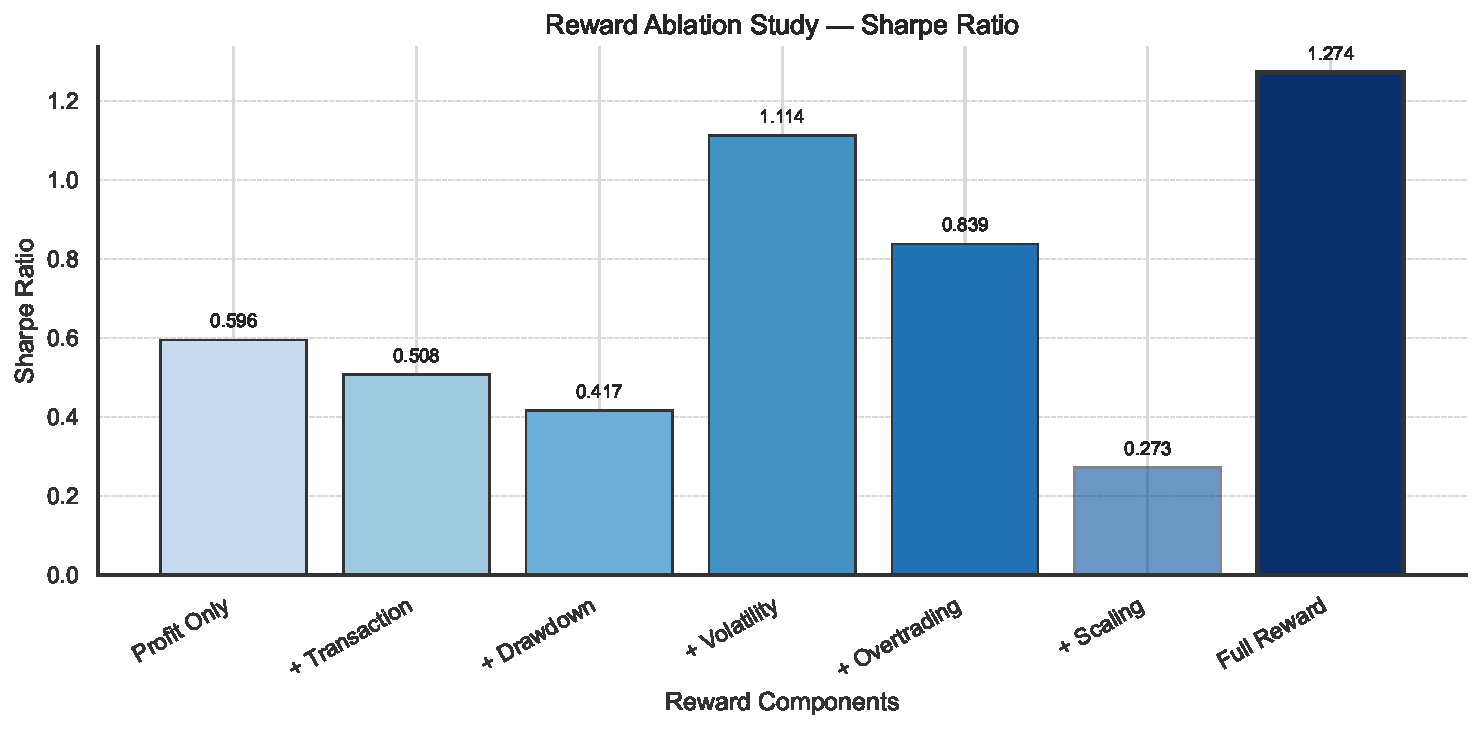
\includegraphics[width=\linewidth]{figures/sharpe_ablation.pdf}
\caption{Reward-ablation comparison for variants \variant{r1}--\variant{r7} on EURUSD, showing a non-monotone profile with \variant{r7} as the strongest endpoint.}
\label{fig:ablation_bar}
\end{figure}

\Cref{fig:ablation_bar} makes the non-monotonicity explicit: the sequence deteriorates from \variant{r1} to \variant{r2}, recovers across \variant{r3}--\variant{r5}, softens at \variant{r6}, and peaks at \variant{r7}.

\begin{figure*}[!tbp]
\centering
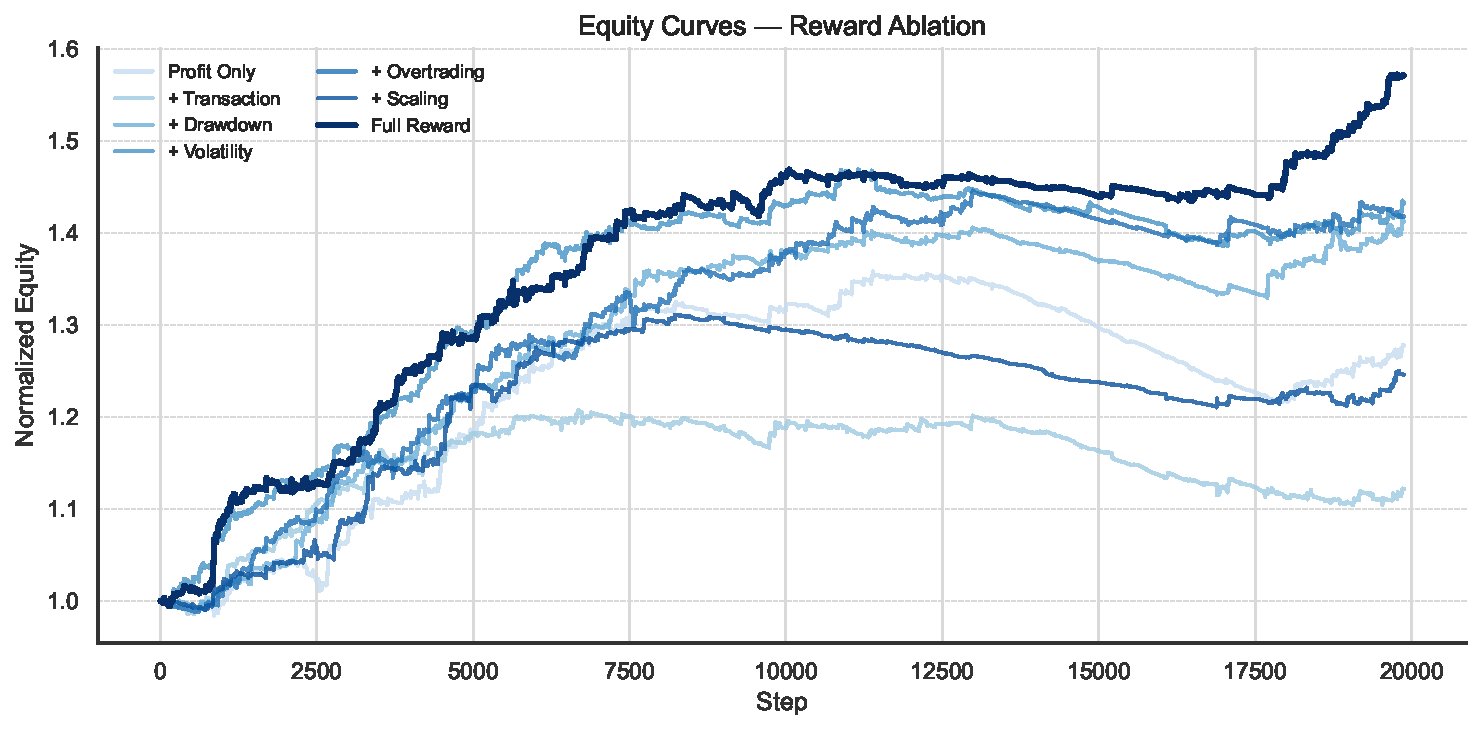
\includegraphics[width=\linewidth]{figures/equity_curves_ablation.pdf}
\caption{Training equity trajectories for \variant{r1}--\variant{r7}, highlighting non-monotone intermediate behavior and the strongest endpoint for \variant{r7}.}
\label{fig:equity_curves_ablation}
\end{figure*}

The trajectory view in \Cref{fig:equity_curves_ablation} corroborates the endpoint summary: the strongest terminal profile is not produced by the earliest penalty additions, but by the fully calibrated composition. This supports the claim that reward engineering is an empirical calibration task rather than a strictly additive design process.

% ------------------------------------------------------------------
\subsection{Action-Space Comparison (\Exp{02})}
% ------------------------------------------------------------------

\noindent\textbf{Objective.}
\Exp{02} compares the extended 10-action interface with the simplified 3-action adapter under matched training settings.

% tab04_action_space.tex
\begin{table}[!tbp]
\centering
\caption{Action-space comparison on EURUSD (Double DQN).}
\label{tab:action_space}
\begin{adjustbox}{width=\linewidth}
\begin{tabular}{@{}lrrrrr@{}}
\toprule
\textbf{Action Space} & \textbf{Sharpe} & \textbf{Cum.Ret(\%)} & \textbf{MaxDD(\%)} & \textbf{WinRate(\%)} & \textbf{Turnover} \\
\midrule
Extended (10) & 0.765 & 57.09 & 2.31 & 33.15 & 1156.51 \\
Simplified (3) & 2.433 & 33.21 & 0.29 & 68.13 & 528.65  \\
\bottomrule
\end{tabular}
\end{adjustbox}
\end{table}




As shown in \Cref{tab:action_space}, the extended interface improves cumulative return while increasing turnover and reducing Sharpe relative to the conservative adapter, indicating a return--activity trade-off under fixed budget.

To visualize how this trade-off accumulates over the episode rather than only at endpoint, \Cref{fig:action_space_equity_comparison} contrasts the corresponding equity paths.

\begin{figure}[!tbp]
\centering
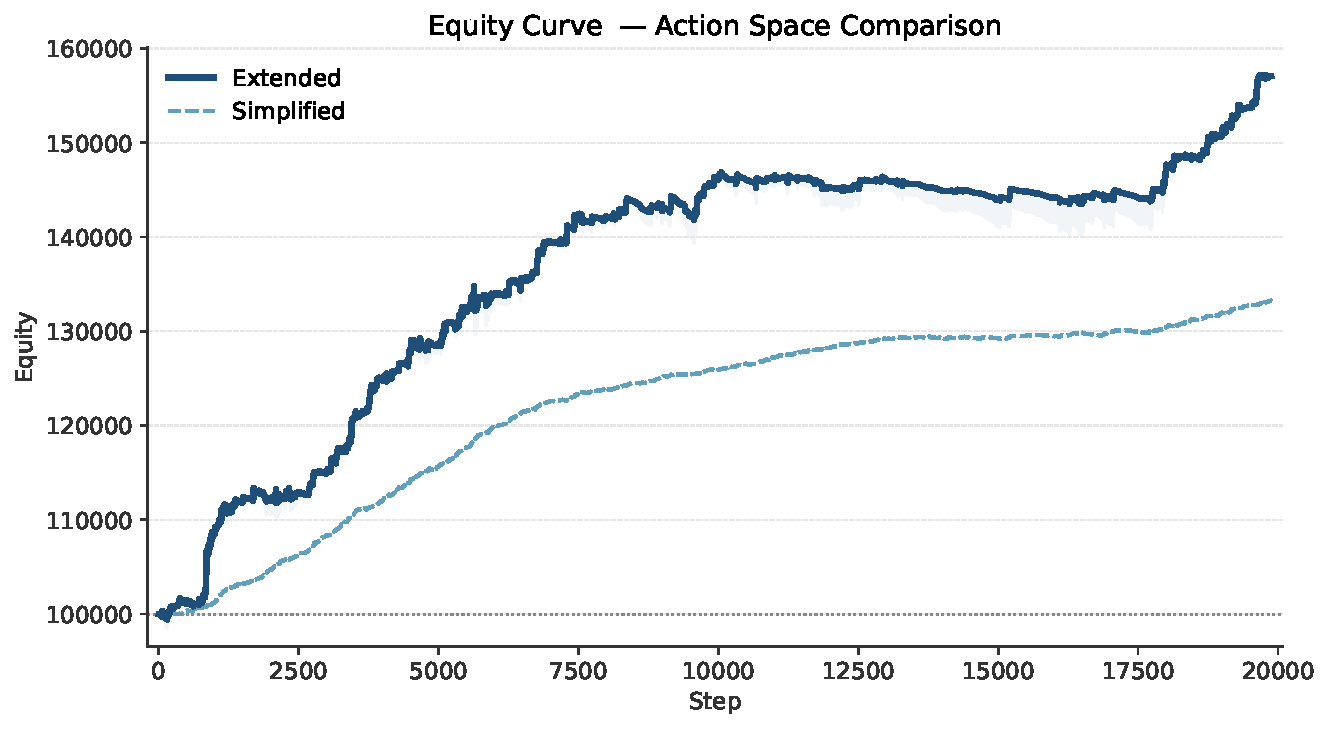
\includegraphics[width=\linewidth]{figures/action_space_equity_comparison.pdf}
\caption{Equity-curve comparison of simplified (3-action) and extended (10-action) interfaces on EURUSD, showing a return--smoothness trade-off.}
\label{fig:action_space_equity_comparison}
\end{figure}

The temporal separation in \Cref{fig:action_space_equity_comparison} clarifies that action granularity changes policy behavior throughout training, not only final-point metrics: richer primitives increase opportunity capture but amplify path variability.

% ------------------------------------------------------------------
\subsection{Scaling Strategy Analysis (\Exp{03})}
% ------------------------------------------------------------------

\noindent\textbf{Objective.}
\Exp{03} evaluates four scaling configurations: no scaling (\variant{s1}), pyramid-only (\variant{s2}), martingale-only (\variant{s3}), and combined (\variant{s4}).

% tab05_scaling.tex
\begin{table}[!tbp]
\centering
\caption{Scaling-strategy analysis on EURUSD (Double DQN).}
\label{tab:scaling}
\begin{adjustbox}{width=\linewidth}
\begin{tabular}{@{}lrrrrrr@{}}
\toprule
\textbf{Variant} & \textbf{Sharpe} & \textbf{Cum.Ret(\%)} & \textbf{MaxDD(\%)} & \textbf{AvgPyr} & \textbf{AvgMart} & \textbf{Turnover} \\
\midrule
s1\_no\_scaling & -1.568 & -16.54 & 16.74 & 0.000 & 0.000 & 1440.09 \\
s2\_pyramid & -0.136 & -2.48 & 5.73 & 0.083 & 0.000 & 1394.52 \\
s3\_martingale & 0.319 & 8.94 & 4.63 & 0.000 & 0.122 & 1273.71 \\
s4\_both & 0.355 & 13.08 & 6.79 & 0.086 & 0.096 & 1483.55 \\
\bottomrule
\end{tabular}
\end{adjustbox}
\end{table}



\Cref{tab:scaling} shows that all scaling-enabled variants improve over no scaling, with distinct objective-dependent preferences across return and drawdown.

\begin{figure}[!tbp]
\centering
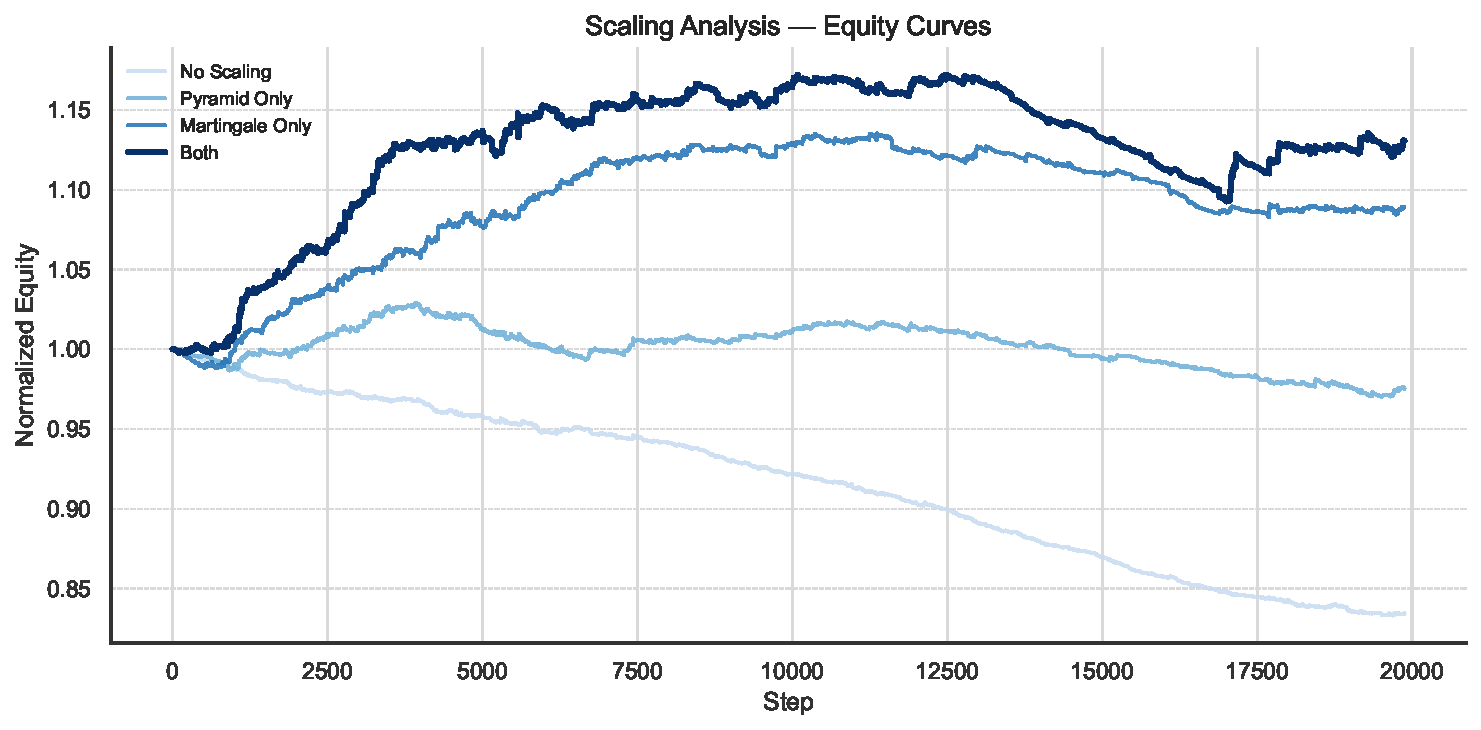
\includegraphics[width=\linewidth]{figures/equity_curves_scaling.pdf}
\caption{Training equity trajectories for scaling variants \variant{s1}--\variant{s4} on EURUSD, where scaling-enabled variants reduce maximum drawdown versus no scaling.}
\label{fig:equity_curves_scaling}
\end{figure}

The path-level evidence in \Cref{fig:equity_curves_scaling} confirms that the gap is structural rather than noise at a single endpoint: enabling scaling alters drawdown dynamics over the full training horizon.

% ------------------------------------------------------------------
\subsection{Benchmark Calibration on EURUSD}
% ------------------------------------------------------------------

% NOTE: All benchmark tables and figures below report results on the EURUSD training split (see Section~\ref{sec:experiments}).
Primary RQ findings are further calibrated against non-RL baselines and a DQN comparator. We first report headline endpoint metrics in \Cref{tab:benchmarks}, then inspect complementary risk diagnostics in \Cref{tab:benchmark_risk}.

\begin{table}[!tbp]
\centering
\caption{Benchmark comparison on EURUSD. RL agents use full reward variant \variant{r7}.}
\label{tab:benchmarks}
\begin{adjustbox}{width=\linewidth}
\begin{tabular}{@{}lrrrrr@{}}
\toprule
\textbf{Method} & \textbf{Sharpe} & \textbf{Cum.Ret(\%)} & \textbf{MaxDD(\%)} & \textbf{WinRate(\%)} & \textbf{Turnover} \\
\midrule
Random Policy & -13.380 & -34.58 & 34.70 & 25.99 & 2199.98 \\
Buy-and-Hold & -0.358 & -1.05 & 2.08 & 0.00 & 0.11 \\
Momentum & -1.355 & -3.82 & 4.05 & 23.62 & 186.28 \\
Mean-Reversion & -0.807 & -1.67 & 2.34 & 24.64 & 157.67 \\
DQN & 0.369 & 24.56 & 8.72 & 34.12 & 1316.51 \\
Double DQN & 0.765 & 57.09 & 2.31 & 33.15 & 1156.51 \\
\bottomrule
\end{tabular}
\end{adjustbox}
\end{table}




\begin{table}[!tbp]
\centering
\caption{Benchmark risk diagnostics on EURUSD (see Section~\ref{sec:experiments}).}
\label{tab:benchmark_risk}
\begin{adjustbox}{width=\linewidth}
\begin{tabular}{@{}lrrrrr@{}}
\toprule
\textbf{Method} & \textbf{Ann.Ret(\%)} & \textbf{Ann.Vol(\%)} & \textbf{Sortino} & \textbf{Trades} \\
\midrule
Random Policy & -12.11 & 0.96 & -16.523 & 13728 \\
Buy-and-Hold & -0.32 & 0.89 & -0.466 & 1 \\
Momentum & -1.18 & 0.87 & -1.789 & 1715 \\
Mean-Reversion & -0.51 & 0.63 & -0.772 & 1469 \\
DQN & 6.36 & 3.37 & 2.643 & 11240 \\
Double DQN & 14.82 & 4.11 & 4.771 & 8415 \\
\bottomrule
\end{tabular}
\end{adjustbox}
\end{table}




Taken together, the two tables show that RL improvements are not merely profit inflation: Double DQN remains favorable under risk-aware summaries and avoids liquidation events in this artifact view, while rule-based baselines underperform on cumulative return.

\begin{figure*}[!tbp]
\centering
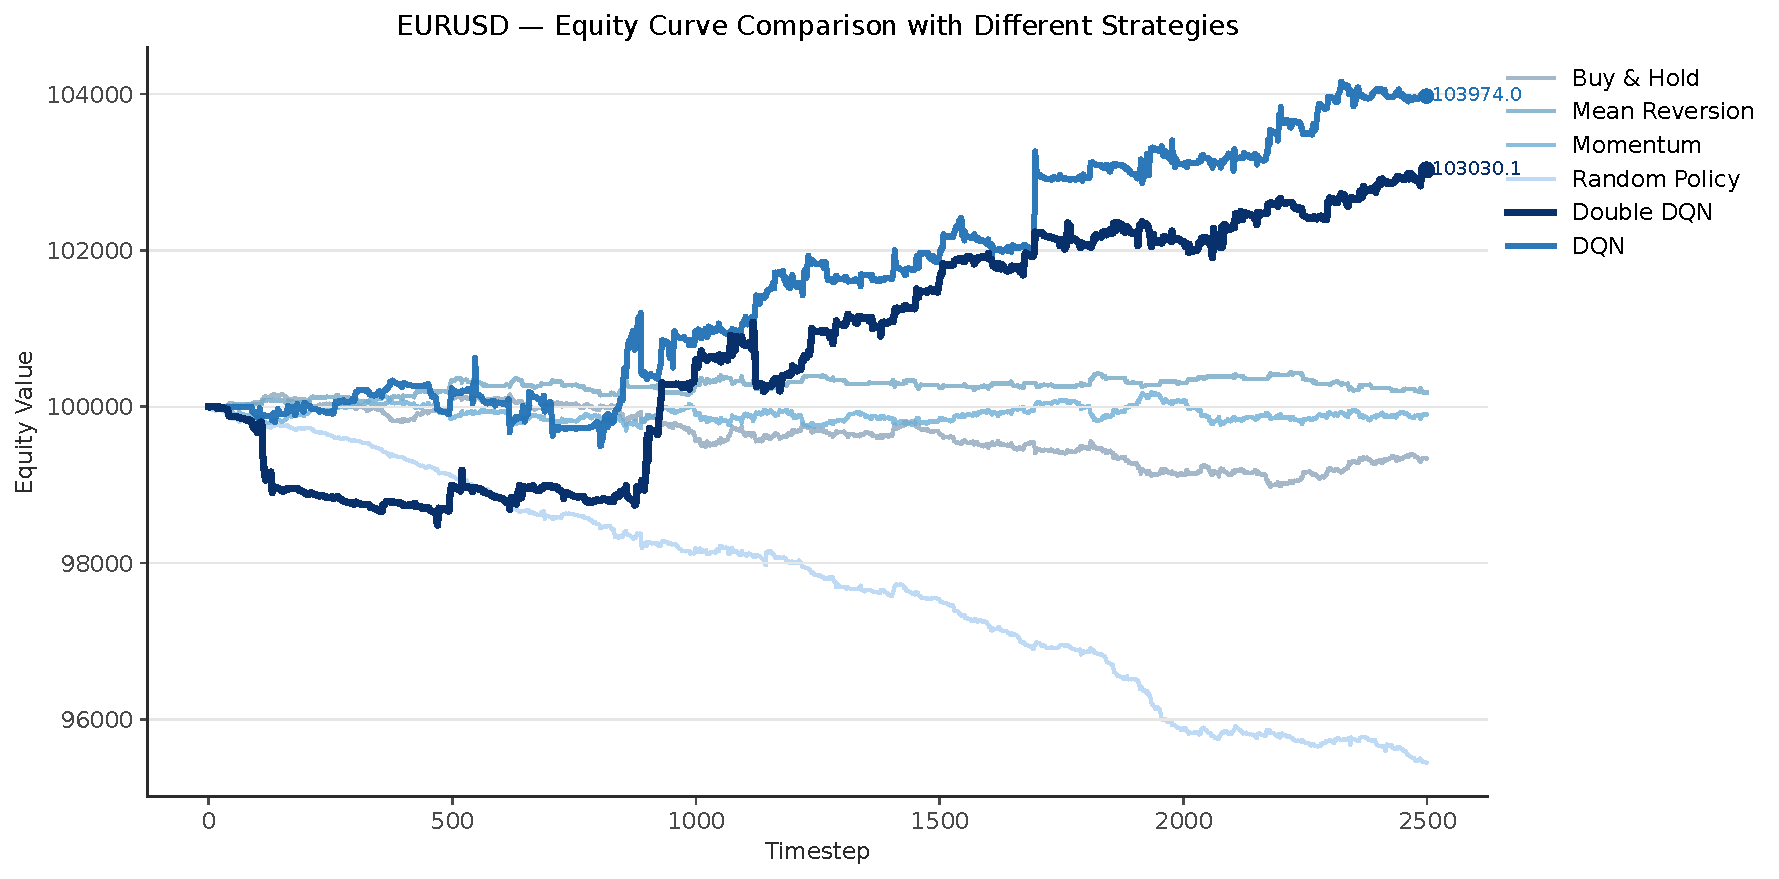
\includegraphics[width=\linewidth]{figures/equity_comparison_with_benmark_startegies.pdf}
\caption{Equity trajectories for RL agents and benchmark strategies on EURUSD, with rule-based baselines as calibration anchors.}
\label{fig:benchmark_equity_comparison}
\end{figure*}

\Cref{fig:benchmark_equity_comparison} reinforces that the learning-based agents maintain stronger growth profiles than benchmark heuristics under identical execution assumptions.

% ------------------------------------------------------------------
\subsection{Cross-Pair Generality Diagnostics}
% ------------------------------------------------------------------

To assess whether the EURUSD pattern is idiosyncratic, \Cref{tab:cross_pair} reports DQN-vs-DDQN outcomes on three additional pairs using the same full-reward configuration.

\begin{table*}[!tbp]
\centering
\caption{Cross-pair DQN vs.\ Double DQN on train split (full reward variant \variant{r7} ).}
\label{tab:cross_pair}

\begin{adjustbox}{width=\linewidth}
\begin{tabular}{llrrrrr}
\toprule
\textbf{Pair} & \textbf{Agent} & \textbf{Sharpe} & \textbf{Sortino} & \textbf{Cum.Ret(\%)} & \textbf{MaxDD(\%)} & \textbf{WinRate(\%)} \\
\midrule
EURUSD & DQN & 0.369 & 0.501 & 24.53 & 8.72 & 34.15 \\
EURUSD & DDQN & 0.765 & 1.117 & 57.09 & 2.31 & 33.15 \\
\midrule
GBPUSD & DQN & 0.164 & 0.195 & 11.98 & 9.59 & 31.96 \\
GBPUSD & DDQN & 0.759 & 0.969 & 83.19 & 3.14 & 31.90 \\
\midrule
USDJPY & DQN & 0.958 & 1.419 & 94.08 & 2.16 & 35.63 \\
USDJPY & DDQN & 1.115 & 1.615 & 115.01 & 4.44 & 33.69 \\
\midrule
AUDUSD & DQN & 0.542 & 0.754 & 33.93 & 7.63 & 30.91 \\
AUDUSD & DDQN & 0.811 & 1.222 & 52.98 & 4.91 & 32.16 \\
\bottomrule
\end{tabular}
\end{adjustbox}
\end{table*}




These results are restricted to the experimental scope defined in Section~\ref{sec:experiments}; the directional trend across pairs is descriptive: Double DQN is generally stronger on return-oriented metrics, with pair-specific differences in drawdown behavior.

\begin{figure*}[!tbp]
\centering
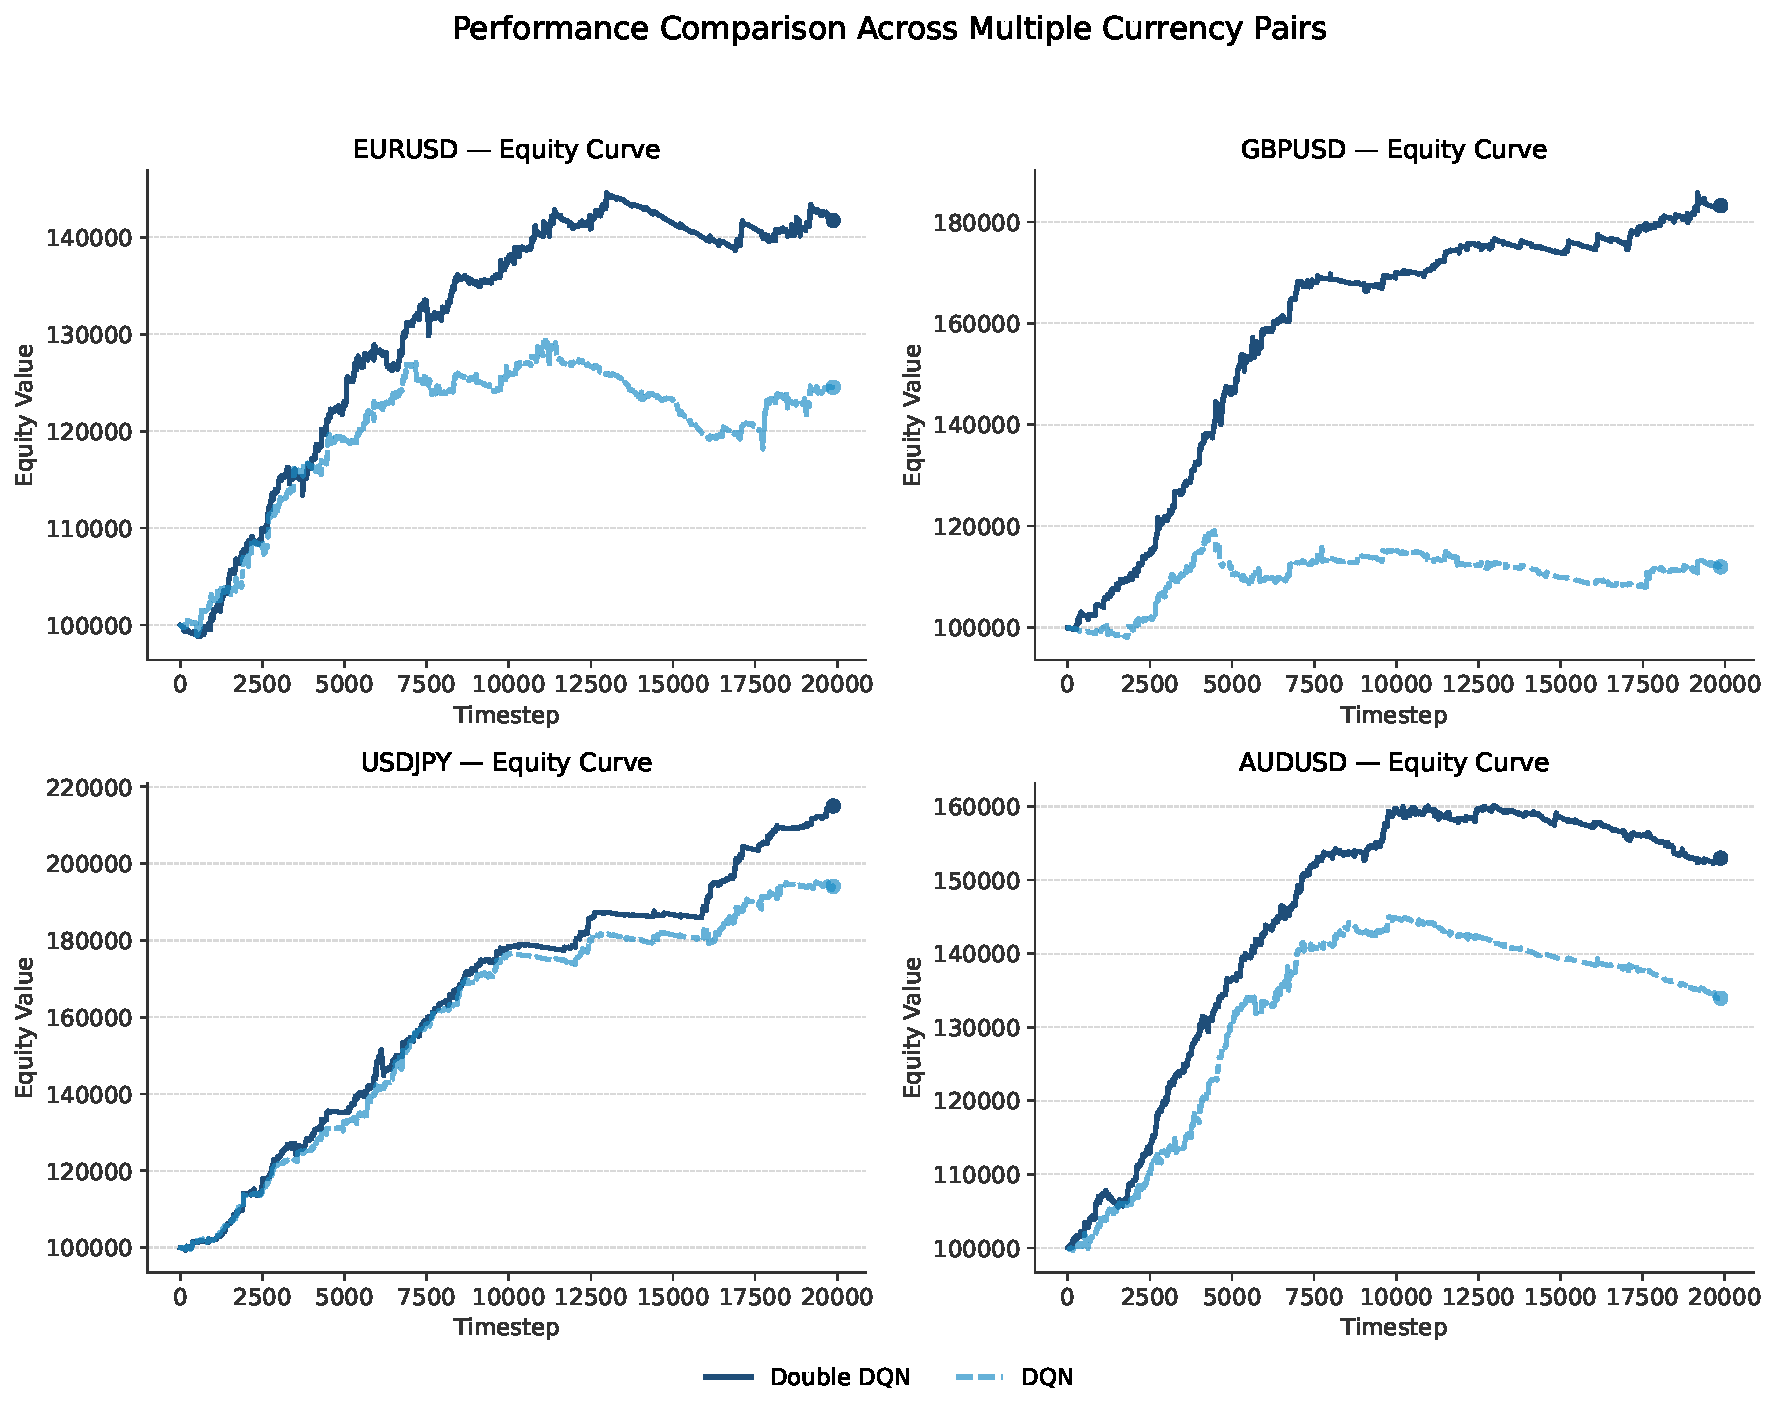
\includegraphics[width=\linewidth]{figures/multi_pair_equity_curves.pdf}
\caption{Multi-pair equity trajectories (EURUSD, GBPUSD, USDJPY, AUDUSD) for value-based agents under aligned simulator and reward settings.}
\label{fig:multi_pair_equity_curves}
\end{figure*}

\Cref{fig:multi_pair_equity_curves} illustrates that cross-pair behavior is heterogeneous in amplitude but consistent in qualitative ordering, supporting the use of pair-diverse diagnostics alongside the primary EURUSD-focused research questions.